% =====================================================================
%  Preview / verification driver for the figure floats in this directory.
% ---------------------------------------------------------------------
%  The figures are `figure*` floats meant for \input into a paper. This
%  driver renders every one of them, in order, on its own page so the
%  set can be eyeballed without a full paper build:
%
%      tectonic -X compile _preview.tex        # -> _preview.pdf
%      # or: pdflatex _preview.tex
%
%  It neutralises the float wrapper (\begin{figure*} .. \caption .. )
%  into a plain centered block so nothing floats to the end of the
%  document; the figure BODIES are rendered exactly as in the paper.
% =====================================================================
\documentclass[11pt]{article}
\usepackage[paperwidth=13in, paperheight=9in, margin=0.5in]{geometry}
\usepackage{tikz}
\usepackage{xcolor}
% =====================================================================
%  Shared preamble for the Hangar architecture / provenance figures.
% ---------------------------------------------------------------------
%  Each figure .tex in this directory is now a bare `figure*` float meant
%  to be \input into a paper (not a standalone document). The TikZ
%  libraries, colour palette, and in-node text macros they all rely on
%  live here so they are defined exactly once.
%
%  In your paper, after \usepackage{tikz} and \usepackage{xcolor}:
%
%      % =====================================================================
%  Shared preamble for the Hangar architecture / provenance figures.
% ---------------------------------------------------------------------
%  Each figure .tex in this directory is now a bare `figure*` float meant
%  to be \input into a paper (not a standalone document). The TikZ
%  libraries, colour palette, and in-node text macros they all rely on
%  live here so they are defined exactly once.
%
%  In your paper, after \usepackage{tikz} and \usepackage{xcolor}:
%
%      % =====================================================================
%  Shared preamble for the Hangar architecture / provenance figures.
% ---------------------------------------------------------------------
%  Each figure .tex in this directory is now a bare `figure*` float meant
%  to be \input into a paper (not a standalone document). The TikZ
%  libraries, colour palette, and in-node text macros they all rely on
%  live here so they are defined exactly once.
%
%  In your paper, after \usepackage{tikz} and \usepackage{xcolor}:
%
%      \input{docs/provenance-figures/_preamble}   % or copy its body
%      ...
%      \input{docs/provenance-figures/omd-provagent-ontology}
%
%  To compile/preview the figures on their own, see _preview.tex.
% =====================================================================

\usetikzlibrary{arrows.meta, positioning, shapes.geometric,
                shapes.multipart, fit, backgrounds, calc}

% --- muted grayscale base --------------------------------------------
\definecolor{ink}{HTML}{1A1A1A}
\definecolor{edge}{HTML}{404040}
\definecolor{muted}{HTML}{6B6B6B}

% --- W3C PROV class palette (prov-metamodel, session-graph, omd-provagent)
\definecolor{entfill}{HTML}{FBF3D3}   % PROV entity   — soft yellow
\definecolor{entline}{HTML}{9C8B33}
\definecolor{actfill}{HTML}{DDE7F7}   % PROV activity — soft blue
\definecolor{actline}{HTML}{3F6FB0}
\definecolor{agtfill}{HTML}{FBE1C0}   % PROV agent    — soft orange
\definecolor{agtline}{HTML}{BE843A}

% --- plan-dag UML section tints --------------------------------------
\definecolor{mslate}{HTML}{C9D4E0}    % Plan (composite)
\definecolor{mblue}{HTML}{DCE7F7}     % model / topology
\definecolor{mamber}{HTML}{FBEFCB}    % optimization problem
\definecolor{mrose}{HTML}{F6DDD9}     % requirements / intent
\definecolor{mgray}{HTML}{E4E7EB}     % analysis process

% --- execution-architecture: leaf analysis tool (soft green) ---------
\definecolor{toolfill}{HTML}{D8E9CF}
\definecolor{toolline}{HTML}{4E8A5E}

% --- shared in-node text switches ------------------------------------
\newcommand{\nattr}{\normalfont\ttfamily\scriptsize\color{muted}}
\newcommand{\nhead}{\normalfont\sffamily\bfseries}
\newcommand{\cn}[1]{\textbf{#1}}                    % UML class name
\newcommand{\at}{\ttfamily\scriptsize\color{muted}} % UML attribute text

% =====================================================================
%  Code-listing style for the plan-YAML figures (ocp-oas-plan-listing).
%  Requires the `listings` package (ships with TeX Live / MiKTeX).
% =====================================================================
\usepackage{listings}
\definecolor{codebg}{HTML}{FAF9F5}    % near-white paper panel

\lstdefinelanguage{planyaml}{
  morecomment=[l]{\#},
  morestring=[b]",
  morestring=[b]',
  alsoletter={_./|},                  % keep dotted/slashed keys as one token
  sensitive=true,
}
% Position-based key colouring: the default (key) style is blueprint-blue
% bold; at each `:` we flip to ink/medium for the value. This colours keys
% by position — not by word — so words like "drag" inside a value string
% are NOT mis-highlighted.
\lstdefinestyle{planyaml}{
  language=planyaml,
  basicstyle=\ttfamily\small\color{actline}\bfseries,
  moredelim=**[l][\color{ink}\mdseries]{:},
  commentstyle=\ttfamily\small\color{toolline}\itshape,
  stringstyle=\color{ink}\mdseries,
  showstringspaces=false,
  keepspaces=true, columns=fullflexible, breaklines=false, tabsize=2,
  frame=single, framesep=5pt, rulecolor=\color{muted},
  backgroundcolor=\color{codebg},
  aboveskip=2pt, belowskip=0pt,
}
   % or copy its body
%      ...
%      % =====================================================================
%  Hangar provenance — Layer 2: the omd PROV-Agent artifact ontology
% ---------------------------------------------------------------------
%  Standalone TikZ figure. Compile with any modern TeX Live:
%
%      pdflatex omd-provagent-ontology.tex
%      latexmk -pdf omd-provagent-ontology.tex     % cropped PDF
%
%  Required packages (all ship with a standard TeX Live / MiKTeX):
%      standalone, tikz (+ libraries below), xcolor
%
%  Visual notation follows W3C PROV (see prov-metamodel-ontology.tex for the
%  abstract base model): Entity = ellipse (soft yellow), Activity = rectangle
%  (soft blue), Agent = pentagon (soft orange). This figure is the concrete
%  instance emitted by ONE omd plan run. Solid edges are PROV relations
%  (core + PROV-Agent domain); dashed edges are agent associations.
%
%  Recommended paper caption: see omd-provagent-caption.md
%
%  Source of truth for the schema + vocabulary:
%      packages/results-reader/src/hangar/results_reader/db.py:46   KNOWN_ENTITY_TYPES
%      packages/results-reader/src/hangar/results_reader/db.py:73   KNOWN_PROV_RELATIONS
%      packages/results-reader/src/hangar/results_reader/db.py:98   _DDL (entities/activities/prov_edges)
%      packages/omd/src/hangar/omd/run.py                           edges emitted per run
%      packages/omd/src/hangar/omd/provenance.py                    Cytoscape builder + version diff
%
%  Node placement is verified collision-free by check_layout.py (key
%  "omd-provagent"); keep the two in sync if you move nodes.
% =====================================================================

\begin{figure*}[t]
\centering

\begin{tikzpicture}[
    scale=0.72, transform shape,
    font=\sffamily,
    >=Stealth,
    % --- PROV class shapes ------------------------------------------
    entity/.style={
        ellipse, draw=entline, line width=0.9pt, fill=entfill,
        text=ink, align=center, inner sep=2pt, font=\sffamily\small,
        minimum width=28mm, minimum height=12mm},
    subent/.style={entity, minimum width=24mm, minimum height=8mm,
        font=\sffamily\footnotesize},
    activity/.style={
        rectangle, draw=actline, line width=0.9pt, fill=actfill,
        text=ink, align=center, inner sep=3pt, font=\sffamily\small,
        minimum width=24mm, minimum height=11mm},
    agent/.style={
        regular polygon, regular polygon sides=5, draw=agtline,
        line width=0.9pt, fill=agtfill, text=ink, inner sep=1pt,
        align=center, font=\sffamily\small, minimum width=22mm},
    % --- relation edge styles: PROV=dark solid, agent assoc=dashed ---
    rel/.style={->, line width=0.8pt, draw=edge},
    agentedge/.style={->, line width=0.7pt, draw=muted, densely dashed},
    rlab/.style={font=\sffamily\scriptsize\itshape, text=ink,
                 fill=white, inner sep=1.4pt, align=center},
]

% ============ agents (top corners) ==================================
\node[agent] (have) at (2.5,7.4)  {coding\\agent};
\node[agent] (omd)  at (13.0,7.5) {omd};

% ============ plan lineage (replan) =================================
\node[entity]   (planA)  at (1.5,4.8)  {plan\\[-1pt]\nattr v($N{-}1$)};
\node[activity] (replan) at (6.0,4.8)  {replan};
\node[entity]   (planB)  at (10.5,4.8) {plan v($N$)\\[-1pt]\nattr content\_hash};

\draw[rel] (replan) -- node[rlab,above]{used} (planA);
\draw[rel] (planB)  -- node[rlab,above]{was\\DerivedFrom} (replan);
% agent associations (dashed): activity->agent = wasAssociatedWith,
% entity->agent = wasAttributedTo (see legend)
\draw[agentedge] (replan.north) to[out=100,in=-120]
      node[rlab,pos=0.5]{was\\AssociatedWith} (have.south);
\draw[agentedge] (planB.north)  to[out=80,in=-135]
      node[rlab,pos=0.42]{was\\AttributedTo} (omd.west);

% ============ plan sub-entities (fan from planB) ====================
\node[subent] (sd) at (15.5,6.2) {surface\_def};
\node[subent] (op) at (15.5,5.0) {operating\_point};
\node[subent] (sc) at (15.5,3.8) {solver\_config};
\node[subent] (os) at (15.5,2.6) {opt\_setup};
\foreach \n in {sd,op,sc,os}{\draw[rel] (\n.west) to[out=180,in=20] (planB.east);}
\node[rlab, text=ink] at (13.0,5.55) {was\\DerivedFrom};

% ============ execution =============================================
\node[activity] (exec) at (10.5,2.4)  {execute};
\node[entity]   (run)  at (10.5,-0.1) {run\_record};
\node[entity, densely dashed, minimum width=28mm, minimum height=9mm]
      (warm) at (5.5,2.4) {prior run\_record};

\draw[rel] (exec) -- node[rlab,left]{used} (planB);
\draw[rel] (run)  -- node[rlab,left]{was\\GeneratedBy} (exec);
\draw[rel] (exec) -- node[rlab,above,align=center]{used\\(warm-start)} (warm);
\draw[agentedge] (exec.east) to[out=15,in=-80]
      node[rlab,pos=0.5]{was\\AssociatedWith} (omd.south);

% ============ result entities (fan from run_record) =================
\node[subent] (aero) at (15.5,1.1)  {aero\_results};
\node[subent] (strc) at (15.5,-0.1) {struct\_results};
\node[subent] (conv) at (15.5,-1.3) {convergence\_info};
\node[subent] (mstr) at (15.5,-2.5) {model\_structure};
\foreach \n in {aero,strc,conv,mstr}{\draw[rel] (\n.west) to[out=180,in=0] (run.east);}
\node[rlab, text=ink] at (13.0,-0.1) {was\\DerivedFrom};

% ============ assessment / verification =============================
\node[activity] (assess) at (6.0,-1.1) {assess};
\node[entity]   (assmt)  at (6.0,-3.4) {assessment};
\node[entity]   (req)    at (1.5,-3.4) {requirement};
\node[entity, minimum width=32mm] (crit) at (1.5,-5.2) {acceptance\\criterion};
\node[entity, minimum width=22mm, minimum height=9mm] (study) at (10.5,-3.0) {study};

\draw[rel] (assess) -- node[rlab,above,pos=0.55]{used} (run);
\draw[rel] (assmt)  -- node[rlab,left]{was\\GeneratedBy} (assess);
\draw[rel] (assmt) -- node[rlab,above,align=center]{verifies\,$\to$\\satisfies\,/\,violates} (req);
\draw[rel] (req)   -- node[rlab,right]{has\_criterion} (crit);
\draw[rel] (run.south) to[out=-90,in=90] node[rlab,right]{partOf} (study.north);

% =====================================================================
%  Vocabulary legend (bottom strip)
% =====================================================================
\node[anchor=north west, align=left, font=\sffamily\scriptsize, text=ink,
      draw=muted, line width=0.5pt, fill=white, rounded corners=2pt,
      inner sep=6pt] at (-4.2,-6.3)
{\textbf{entity\_type}\ \footnotesize(\texttt{KNOWN\_ENTITY\_TYPES})\\[2pt]
 \ttfamily\scriptsize plan $\cdot$ run\_record $\cdot$ assessment $\cdot$ surface\_def $\cdot$ operating\_point $\cdot$ solver\_config $\cdot$ opt\_setup\\
 \ttfamily\scriptsize aero\_results $\cdot$ struct\_results $\cdot$ convergence\_info $\cdot$ model\_structure $\cdot$ phase $\cdot$ requirement\\
 \ttfamily\scriptsize acceptance\_criterion $\cdot$ plan\_element $\cdot$ decision $\cdot$ conclusion $\cdot$ study\\[5pt]
 \textbf{activity\_type}\ \ttfamily\scriptsize execute $\cdot$ assess $\cdot$ replan\qquad
 \normalfont\textbf{agent}\ \ttfamily\scriptsize omd $\cdot$ coding agent};

\node[anchor=north west, align=left, font=\sffamily\scriptsize, text=ink,
      draw=muted, line width=0.5pt, fill=white, rounded corners=2pt,
      inner sep=6pt] at (9.1,-6.3)
{\textbf{relation}\ \footnotesize(\texttt{KNOWN\_PROV\_RELATIONS})\\[3pt]
 \tikz\draw[rel](0,0)--(0.55,0);\ PROV core:\ \ttfamily\scriptsize wasGeneratedBy $\cdot$ used $\cdot$ wasDerivedFrom\\
 \hspace*{4.3em}\ttfamily\scriptsize wasInformedBy\\[2pt]
 \tikz\draw[rel](0,0)--(0.55,0);\ domain:\ \ttfamily\scriptsize justifies $\cdot$ has\_criterion $\cdot$ verifies $\cdot$ satisfies\\
 \hspace*{4.3em}\ttfamily\scriptsize violates $\cdot$ precedes $\cdot$ has\_check $\cdot$ executes $\cdot$ partOf\\[2pt]
 \tikz\draw[agentedge](0,0)--(0.55,0);\ agent:\ \ttfamily\scriptsize wasAssociatedWith $\cdot$ wasAttributedTo};

\end{tikzpicture}

\caption{Layer~2 --- the \texttt{omd} PROV-Agent artifact ontology (one plan run).}
\label{fig:omd-provagent-ontology}
\end{figure*}

%
%  To compile/preview the figures on their own, see _preview.tex.
% =====================================================================

\usetikzlibrary{arrows.meta, positioning, shapes.geometric,
                shapes.multipart, fit, backgrounds, calc}

% --- muted grayscale base --------------------------------------------
\definecolor{ink}{HTML}{1A1A1A}
\definecolor{edge}{HTML}{404040}
\definecolor{muted}{HTML}{6B6B6B}

% --- W3C PROV class palette (prov-metamodel, session-graph, omd-provagent)
\definecolor{entfill}{HTML}{FBF3D3}   % PROV entity   — soft yellow
\definecolor{entline}{HTML}{9C8B33}
\definecolor{actfill}{HTML}{DDE7F7}   % PROV activity — soft blue
\definecolor{actline}{HTML}{3F6FB0}
\definecolor{agtfill}{HTML}{FBE1C0}   % PROV agent    — soft orange
\definecolor{agtline}{HTML}{BE843A}

% --- plan-dag UML section tints --------------------------------------
\definecolor{mslate}{HTML}{C9D4E0}    % Plan (composite)
\definecolor{mblue}{HTML}{DCE7F7}     % model / topology
\definecolor{mamber}{HTML}{FBEFCB}    % optimization problem
\definecolor{mrose}{HTML}{F6DDD9}     % requirements / intent
\definecolor{mgray}{HTML}{E4E7EB}     % analysis process

% --- execution-architecture: leaf analysis tool (soft green) ---------
\definecolor{toolfill}{HTML}{D8E9CF}
\definecolor{toolline}{HTML}{4E8A5E}

% --- shared in-node text switches ------------------------------------
\newcommand{\nattr}{\normalfont\ttfamily\scriptsize\color{muted}}
\newcommand{\nhead}{\normalfont\sffamily\bfseries}
\newcommand{\cn}[1]{\textbf{#1}}                    % UML class name
\newcommand{\at}{\ttfamily\scriptsize\color{muted}} % UML attribute text

% =====================================================================
%  Code-listing style for the plan-YAML figures (ocp-oas-plan-listing).
%  Requires the `listings` package (ships with TeX Live / MiKTeX).
% =====================================================================
\usepackage{listings}
\definecolor{codebg}{HTML}{FAF9F5}    % near-white paper panel

\lstdefinelanguage{planyaml}{
  morecomment=[l]{\#},
  morestring=[b]",
  morestring=[b]',
  alsoletter={_./|},                  % keep dotted/slashed keys as one token
  sensitive=true,
}
% Position-based key colouring: the default (key) style is blueprint-blue
% bold; at each `:` we flip to ink/medium for the value. This colours keys
% by position — not by word — so words like "drag" inside a value string
% are NOT mis-highlighted.
\lstdefinestyle{planyaml}{
  language=planyaml,
  basicstyle=\ttfamily\small\color{actline}\bfseries,
  moredelim=**[l][\color{ink}\mdseries]{:},
  commentstyle=\ttfamily\small\color{toolline}\itshape,
  stringstyle=\color{ink}\mdseries,
  showstringspaces=false,
  keepspaces=true, columns=fullflexible, breaklines=false, tabsize=2,
  frame=single, framesep=5pt, rulecolor=\color{muted},
  backgroundcolor=\color{codebg},
  aboveskip=2pt, belowskip=0pt,
}
   % or copy its body
%      ...
%      % =====================================================================
%  Hangar provenance — Layer 2: the omd PROV-Agent artifact ontology
% ---------------------------------------------------------------------
%  Standalone TikZ figure. Compile with any modern TeX Live:
%
%      pdflatex omd-provagent-ontology.tex
%      latexmk -pdf omd-provagent-ontology.tex     % cropped PDF
%
%  Required packages (all ship with a standard TeX Live / MiKTeX):
%      standalone, tikz (+ libraries below), xcolor
%
%  Visual notation follows W3C PROV (see prov-metamodel-ontology.tex for the
%  abstract base model): Entity = ellipse (soft yellow), Activity = rectangle
%  (soft blue), Agent = pentagon (soft orange). This figure is the concrete
%  instance emitted by ONE omd plan run. Solid edges are PROV relations
%  (core + PROV-Agent domain); dashed edges are agent associations.
%
%  Recommended paper caption: see omd-provagent-caption.md
%
%  Source of truth for the schema + vocabulary:
%      packages/results-reader/src/hangar/results_reader/db.py:46   KNOWN_ENTITY_TYPES
%      packages/results-reader/src/hangar/results_reader/db.py:73   KNOWN_PROV_RELATIONS
%      packages/results-reader/src/hangar/results_reader/db.py:98   _DDL (entities/activities/prov_edges)
%      packages/omd/src/hangar/omd/run.py                           edges emitted per run
%      packages/omd/src/hangar/omd/provenance.py                    Cytoscape builder + version diff
%
%  Node placement is verified collision-free by check_layout.py (key
%  "omd-provagent"); keep the two in sync if you move nodes.
% =====================================================================

\begin{figure*}[t]
\centering

\begin{tikzpicture}[
    scale=0.72, transform shape,
    font=\sffamily,
    >=Stealth,
    % --- PROV class shapes ------------------------------------------
    entity/.style={
        ellipse, draw=entline, line width=0.9pt, fill=entfill,
        text=ink, align=center, inner sep=2pt, font=\sffamily\small,
        minimum width=28mm, minimum height=12mm},
    subent/.style={entity, minimum width=24mm, minimum height=8mm,
        font=\sffamily\footnotesize},
    activity/.style={
        rectangle, draw=actline, line width=0.9pt, fill=actfill,
        text=ink, align=center, inner sep=3pt, font=\sffamily\small,
        minimum width=24mm, minimum height=11mm},
    agent/.style={
        regular polygon, regular polygon sides=5, draw=agtline,
        line width=0.9pt, fill=agtfill, text=ink, inner sep=1pt,
        align=center, font=\sffamily\small, minimum width=22mm},
    % --- relation edge styles: PROV=dark solid, agent assoc=dashed ---
    rel/.style={->, line width=0.8pt, draw=edge},
    agentedge/.style={->, line width=0.7pt, draw=muted, densely dashed},
    rlab/.style={font=\sffamily\scriptsize\itshape, text=ink,
                 fill=white, inner sep=1.4pt, align=center},
]

% ============ agents (top corners) ==================================
\node[agent] (have) at (2.5,7.4)  {coding\\agent};
\node[agent] (omd)  at (13.0,7.5) {omd};

% ============ plan lineage (replan) =================================
\node[entity]   (planA)  at (1.5,4.8)  {plan\\[-1pt]\nattr v($N{-}1$)};
\node[activity] (replan) at (6.0,4.8)  {replan};
\node[entity]   (planB)  at (10.5,4.8) {plan v($N$)\\[-1pt]\nattr content\_hash};

\draw[rel] (replan) -- node[rlab,above]{used} (planA);
\draw[rel] (planB)  -- node[rlab,above]{was\\DerivedFrom} (replan);
% agent associations (dashed): activity->agent = wasAssociatedWith,
% entity->agent = wasAttributedTo (see legend)
\draw[agentedge] (replan.north) to[out=100,in=-120]
      node[rlab,pos=0.5]{was\\AssociatedWith} (have.south);
\draw[agentedge] (planB.north)  to[out=80,in=-135]
      node[rlab,pos=0.42]{was\\AttributedTo} (omd.west);

% ============ plan sub-entities (fan from planB) ====================
\node[subent] (sd) at (15.5,6.2) {surface\_def};
\node[subent] (op) at (15.5,5.0) {operating\_point};
\node[subent] (sc) at (15.5,3.8) {solver\_config};
\node[subent] (os) at (15.5,2.6) {opt\_setup};
\foreach \n in {sd,op,sc,os}{\draw[rel] (\n.west) to[out=180,in=20] (planB.east);}
\node[rlab, text=ink] at (13.0,5.55) {was\\DerivedFrom};

% ============ execution =============================================
\node[activity] (exec) at (10.5,2.4)  {execute};
\node[entity]   (run)  at (10.5,-0.1) {run\_record};
\node[entity, densely dashed, minimum width=28mm, minimum height=9mm]
      (warm) at (5.5,2.4) {prior run\_record};

\draw[rel] (exec) -- node[rlab,left]{used} (planB);
\draw[rel] (run)  -- node[rlab,left]{was\\GeneratedBy} (exec);
\draw[rel] (exec) -- node[rlab,above,align=center]{used\\(warm-start)} (warm);
\draw[agentedge] (exec.east) to[out=15,in=-80]
      node[rlab,pos=0.5]{was\\AssociatedWith} (omd.south);

% ============ result entities (fan from run_record) =================
\node[subent] (aero) at (15.5,1.1)  {aero\_results};
\node[subent] (strc) at (15.5,-0.1) {struct\_results};
\node[subent] (conv) at (15.5,-1.3) {convergence\_info};
\node[subent] (mstr) at (15.5,-2.5) {model\_structure};
\foreach \n in {aero,strc,conv,mstr}{\draw[rel] (\n.west) to[out=180,in=0] (run.east);}
\node[rlab, text=ink] at (13.0,-0.1) {was\\DerivedFrom};

% ============ assessment / verification =============================
\node[activity] (assess) at (6.0,-1.1) {assess};
\node[entity]   (assmt)  at (6.0,-3.4) {assessment};
\node[entity]   (req)    at (1.5,-3.4) {requirement};
\node[entity, minimum width=32mm] (crit) at (1.5,-5.2) {acceptance\\criterion};
\node[entity, minimum width=22mm, minimum height=9mm] (study) at (10.5,-3.0) {study};

\draw[rel] (assess) -- node[rlab,above,pos=0.55]{used} (run);
\draw[rel] (assmt)  -- node[rlab,left]{was\\GeneratedBy} (assess);
\draw[rel] (assmt) -- node[rlab,above,align=center]{verifies\,$\to$\\satisfies\,/\,violates} (req);
\draw[rel] (req)   -- node[rlab,right]{has\_criterion} (crit);
\draw[rel] (run.south) to[out=-90,in=90] node[rlab,right]{partOf} (study.north);

% =====================================================================
%  Vocabulary legend (bottom strip)
% =====================================================================
\node[anchor=north west, align=left, font=\sffamily\scriptsize, text=ink,
      draw=muted, line width=0.5pt, fill=white, rounded corners=2pt,
      inner sep=6pt] at (-4.2,-6.3)
{\textbf{entity\_type}\ \footnotesize(\texttt{KNOWN\_ENTITY\_TYPES})\\[2pt]
 \ttfamily\scriptsize plan $\cdot$ run\_record $\cdot$ assessment $\cdot$ surface\_def $\cdot$ operating\_point $\cdot$ solver\_config $\cdot$ opt\_setup\\
 \ttfamily\scriptsize aero\_results $\cdot$ struct\_results $\cdot$ convergence\_info $\cdot$ model\_structure $\cdot$ phase $\cdot$ requirement\\
 \ttfamily\scriptsize acceptance\_criterion $\cdot$ plan\_element $\cdot$ decision $\cdot$ conclusion $\cdot$ study\\[5pt]
 \textbf{activity\_type}\ \ttfamily\scriptsize execute $\cdot$ assess $\cdot$ replan\qquad
 \normalfont\textbf{agent}\ \ttfamily\scriptsize omd $\cdot$ coding agent};

\node[anchor=north west, align=left, font=\sffamily\scriptsize, text=ink,
      draw=muted, line width=0.5pt, fill=white, rounded corners=2pt,
      inner sep=6pt] at (9.1,-6.3)
{\textbf{relation}\ \footnotesize(\texttt{KNOWN\_PROV\_RELATIONS})\\[3pt]
 \tikz\draw[rel](0,0)--(0.55,0);\ PROV core:\ \ttfamily\scriptsize wasGeneratedBy $\cdot$ used $\cdot$ wasDerivedFrom\\
 \hspace*{4.3em}\ttfamily\scriptsize wasInformedBy\\[2pt]
 \tikz\draw[rel](0,0)--(0.55,0);\ domain:\ \ttfamily\scriptsize justifies $\cdot$ has\_criterion $\cdot$ verifies $\cdot$ satisfies\\
 \hspace*{4.3em}\ttfamily\scriptsize violates $\cdot$ precedes $\cdot$ has\_check $\cdot$ executes $\cdot$ partOf\\[2pt]
 \tikz\draw[agentedge](0,0)--(0.55,0);\ agent:\ \ttfamily\scriptsize wasAssociatedWith $\cdot$ wasAttributedTo};

\end{tikzpicture}

\caption{Layer~2 --- the \texttt{omd} PROV-Agent artifact ontology (one plan run).}
\label{fig:omd-provagent-ontology}
\end{figure*}

%
%  To compile/preview the figures on their own, see _preview.tex.
% =====================================================================

\usetikzlibrary{arrows.meta, positioning, shapes.geometric,
                shapes.multipart, fit, backgrounds, calc}

% --- muted grayscale base --------------------------------------------
\definecolor{ink}{HTML}{1A1A1A}
\definecolor{edge}{HTML}{404040}
\definecolor{muted}{HTML}{6B6B6B}

% --- W3C PROV class palette (prov-metamodel, session-graph, omd-provagent)
\definecolor{entfill}{HTML}{FBF3D3}   % PROV entity   — soft yellow
\definecolor{entline}{HTML}{9C8B33}
\definecolor{actfill}{HTML}{DDE7F7}   % PROV activity — soft blue
\definecolor{actline}{HTML}{3F6FB0}
\definecolor{agtfill}{HTML}{FBE1C0}   % PROV agent    — soft orange
\definecolor{agtline}{HTML}{BE843A}

% --- plan-dag UML section tints --------------------------------------
\definecolor{mslate}{HTML}{C9D4E0}    % Plan (composite)
\definecolor{mblue}{HTML}{DCE7F7}     % model / topology
\definecolor{mamber}{HTML}{FBEFCB}    % optimization problem
\definecolor{mrose}{HTML}{F6DDD9}     % requirements / intent
\definecolor{mgray}{HTML}{E4E7EB}     % analysis process

% --- execution-architecture: leaf analysis tool (soft green) ---------
\definecolor{toolfill}{HTML}{D8E9CF}
\definecolor{toolline}{HTML}{4E8A5E}

% --- shared in-node text switches ------------------------------------
\newcommand{\nattr}{\normalfont\ttfamily\scriptsize\color{muted}}
\newcommand{\nhead}{\normalfont\sffamily\bfseries}
\newcommand{\cn}[1]{\textbf{#1}}                    % UML class name
\newcommand{\at}{\ttfamily\scriptsize\color{muted}} % UML attribute text

% =====================================================================
%  Code-listing style for the plan-YAML figures (ocp-oas-plan-listing).
%  Requires the `listings` package (ships with TeX Live / MiKTeX).
% =====================================================================
\usepackage{listings}
\definecolor{codebg}{HTML}{FAF9F5}    % near-white paper panel

\lstdefinelanguage{planyaml}{
  morecomment=[l]{\#},
  morestring=[b]",
  morestring=[b]',
  alsoletter={_./|},                  % keep dotted/slashed keys as one token
  sensitive=true,
}
% Position-based key colouring: the default (key) style is blueprint-blue
% bold; at each `:` we flip to ink/medium for the value. This colours keys
% by position — not by word — so words like "drag" inside a value string
% are NOT mis-highlighted.
\lstdefinestyle{planyaml}{
  language=planyaml,
  basicstyle=\ttfamily\small\color{actline}\bfseries,
  moredelim=**[l][\color{ink}\mdseries]{:},
  commentstyle=\ttfamily\small\color{toolline}\itshape,
  stringstyle=\color{ink}\mdseries,
  showstringspaces=false,
  keepspaces=true, columns=fullflexible, breaklines=false, tabsize=2,
  frame=single, framesep=5pt, rulecolor=\color{muted},
  backgroundcolor=\color{codebg},
  aboveskip=2pt, belowskip=0pt,
}

\pagestyle{empty}

% Turn each float into an in-place centered block for preview.
\renewenvironment{figure*}[1][]{\par\begin{center}}{\end{center}\clearpage}
\renewenvironment{figure}[1][]{\par\begin{center}}{\end{center}\clearpage}
\renewcommand{\caption}[1]{\par\smallskip\begin{minipage}{0.8\linewidth}%
  \small\itshape #1\end{minipage}}
\renewcommand{\label}[1]{}

\begin{document}
% =====================================================================
%  W3C PROV / PROV-Agent meta-model (the abstract base ontology)
% ---------------------------------------------------------------------
%  Standalone TikZ figure. Compile with any modern TeX Live:
%
%      pdflatex prov-metamodel-ontology.tex
%      latexmk -pdf prov-metamodel-ontology.tex     % cropped PDF
%
%  Required packages (all ship with a standard TeX Live / MiKTeX):
%      standalone, tikz (+ libraries below), xcolor
%
%  Visual notation follows W3C PROV, with the conventional PROV class
%  colours (muted for print):
%      Entity   = ellipse   (soft yellow)
%      Activity = rectangle (soft blue)
%      Agent    = pentagon  (soft orange)
%
%  This is the generic model that Layer 2 (omd-provagent-ontology.tex)
%  instantiates and extends with domain relations. PROV-Agent adds the
%  agent-centric associations for agentic AI workflows (arXiv:2508.02866).
%
%  Recommended paper caption: see prov-metamodel-caption.md
% =====================================================================
\documentclass[border=10pt]{standalone}

\usepackage{xcolor}
\usepackage{tikz}
\usetikzlibrary{arrows.meta, positioning, shapes.geometric, calc}

% --- palette: muted grayscale base + conventional PROV class colours ---
\definecolor{ink}{HTML}{1A1A1A}
\definecolor{edge}{HTML}{404040}
\definecolor{muted}{HTML}{6B6B6B}
\definecolor{entfill}{HTML}{FBF3D3}   % PROV entity   — soft yellow
\definecolor{entline}{HTML}{9C8B33}
\definecolor{actfill}{HTML}{DDE7F7}   % PROV activity — soft blue
\definecolor{actline}{HTML}{3F6FB0}
\definecolor{agtfill}{HTML}{FBE1C0}   % PROV agent    — soft orange
\definecolor{agtline}{HTML}{BE843A}

% --- output size: ONE knob. Rescales the whole figure (shapes + text)
%     uniformly. Default 0.7 emits a compact PDF; set 1.0 for full size.
%     In the paper you can instead size it at include time, e.g.
%       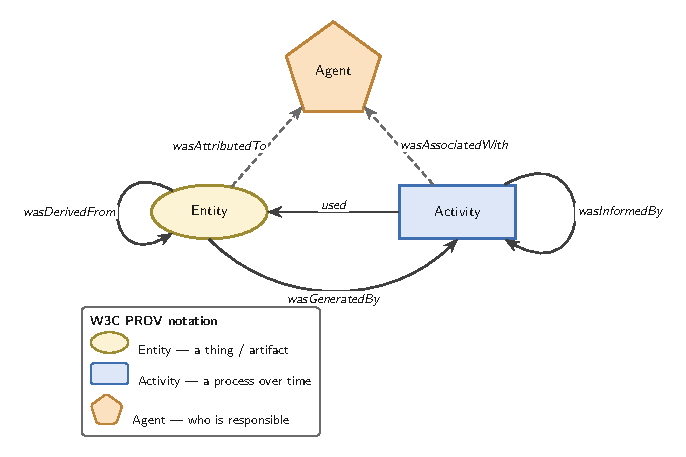
\includegraphics[width=0.7\textwidth]{prov-metamodel-ontology}
\newcommand{\figscale}{0.7}

\begin{document}
\begin{tikzpicture}[
    scale=\figscale, transform shape,
    font=\sffamily,
    >=Stealth,
    entity/.style={
        ellipse, draw=entline, line width=0.9pt, fill=entfill,
        text=ink, align=center, inner sep=2pt, font=\sffamily,
        minimum width=28mm, minimum height=13mm},
    activity/.style={
        rectangle, draw=actline, line width=0.9pt, fill=actfill,
        text=ink, align=center, inner sep=3pt, font=\sffamily,
        minimum width=28mm, minimum height=13mm},
    agent/.style={
        regular polygon, regular polygon sides=5, draw=agtline,
        line width=0.9pt, fill=agtfill, text=ink, inner sep=1pt,
        font=\sffamily, minimum width=24mm},
    rel/.style={->, line width=0.8pt, draw=edge},
    aedge/.style={->, line width=0.7pt, draw=muted, densely dashed},
    lab/.style={font=\sffamily\small\itshape, text=ink,
                fill=white, inner sep=1.6pt},
]

% --- the three PROV classes ------------------------------------------
\node[entity]   (E) at (0,0)   {Entity};
\node[activity] (A) at (6,0)   {Activity};
\node[agent]    (G) at (3,3.4) {Agent};

% --- the six core relations ------------------------------------------
% used: activity used an entity
\draw[rel] (A) -- node[lab,above]{used} (E);
% wasGeneratedBy: entity generated by activity (arc below)
\draw[rel] (E.south) to[out=-45,in=-135]
           node[lab,below]{wasGeneratedBy} (A.south);
% wasDerivedFrom: entity from entity (self-loop, left)
\draw[rel] (E) to[out=150,in=210,looseness=5]
           node[lab,left]{wasDerivedFrom} (E);
% wasInformedBy: activity from activity (self-loop, right)
\draw[rel] (A) to[out=30,in=-30,looseness=5]
           node[lab,right]{wasInformedBy} (A);
% agent associations (dashed)
\draw[aedge] (A) -- node[lab,pos=0.52,right]{wasAssociatedWith} (G);
\draw[aedge] (E) -- node[lab,pos=0.52,left]{wasAttributedTo} (G);

% --- shape key (compact, lower strip) --------------------------------
\node[anchor=north west, align=left, font=\sffamily\small, text=ink,
      draw=muted, line width=0.5pt, rounded corners=2pt, inner sep=6pt]
      at (-3.1,-2.3)
{\textbf{W3C PROV notation}\\[3pt]
 \tikz\node[entity,minimum width=9mm,minimum height=5mm,inner sep=0pt]{};\ \ Entity — a thing / artifact\\[3pt]
 \tikz\node[activity,minimum width=9mm,minimum height=5mm,inner sep=0pt]{};\ \ Activity — a process over time\\[3pt]
 \tikz\node[agent,minimum width=8mm,inner sep=0pt]{};\ \ Agent — who is responsible};

\end{tikzpicture}
\end{document}

% =====================================================================
%  Hangar provenance — Layer 1: the @capture_tool session-graph ontology
% ---------------------------------------------------------------------
%  Standalone TikZ figure. Compile with any modern TeX Live:
%
%      pdflatex session-graph-ontology.tex
%      latexmk -pdf session-graph-ontology.tex     % cropped PDF
%
%  Required packages (all ship with a standard TeX Live / MiKTeX):
%      standalone, tikz (+ libraries below), xcolor
%
%  Notation follows W3C PROV (see prov-metamodel-ontology.tex): Entity =
%  ellipse (soft yellow), Activity = rectangle (soft blue), Agent =
%  pentagon (soft orange), Session = Bundle (dashed enclosure). Layer 1 is
%  a *lighter* call/decision trace, not full PROV (doc S5): it is
%  activity-centric (tool calls + decisions are activities; requirement is
%  the only entity), most edges are INFERRED from seq order, and the LLM is
%  NOT a stored first-class agent — hence the agent is drawn dashed/implicit.
%  The edge labels keep the schema's own names; the legend maps each to its
%  notional PROV relation.
%
%  Recommended paper caption: see session-graph-caption.md
%
%  Source of truth for the schema:
%      packages/sdk/src/hangar/sdk/provenance/db.py      (DDL, 5 tables)
%      packages/sdk/src/hangar/sdk/provenance/db.py:487  (get_session_graph,
%                                                          edge inference)
%      packages/sdk/src/hangar/sdk/provenance/tools.py   (agent-authored tools)
%      packages/sdk/src/hangar/sdk/provenance/conclusion.py (auto verdicts)
% =====================================================================

\begin{figure*}[t]
\centering

\begin{tikzpicture}[
    scale=0.75, transform shape,
    font=\sffamily,
    >=Stealth,
    % --- PROV class shapes ------------------------------------------
    activity/.style={
        rectangle, rounded corners=1pt, draw=actline, line width=0.9pt,
        fill=actfill, inner sep=4pt, align=left, text=ink, minimum width=33mm},
    entity/.style={
        ellipse, draw=entline, line width=0.9pt, fill=entfill, align=center,
        text=ink, inner sep=1pt, minimum width=44mm, minimum height=20mm},
    agent/.style={
        regular polygon, regular polygon sides=5, draw=agtline, densely dashed,
        line width=0.9pt, fill=agtfill, text=ink, inner sep=1pt,
        align=center, minimum width=22mm},
    % --- edge styles: solid=stored, dashed=inferred, dotted=agent assoc
    stored/.style={->, draw=ink, line width=1.0pt},
    inferred/.style={->, draw=muted, dashed, line width=0.9pt},
    assoc/.style={->, draw=muted, densely dotted, line width=0.7pt},
    elabel/.style={font=\sffamily\scriptsize\itshape, text=ink,
                   fill=white, inner sep=1.5pt, align=center},
]

% ============ agent (implicit — not stored in Layer 1) ==============
\node[agent, minimum width=18mm] (agent) at (12.7,4.8) {agent\\[-1pt]\nattr (runtime/user)};

% ============ the temporal call / decision trace ====================
\node[activity] (t1) at (1.0,2.4)
    {{\nhead ToolCall}\,\nattr(seq $n$)\\[1pt]
     \nattr call\_id, tool\_name\\
     \nattr inputs\_json / outputs\_json\\
     \nattr status, duration\_s};

\node[activity] (d1) at (6.5,2.4)
    {{\nhead Decision}\\[1pt]
     \nattr decision\_type\\
     \nattr reasoning, selected\_action\\
     \nattr prior\_call\_id, confidence};

\node[activity] (t2) at (12.0,2.4)
    {{\nhead ToolCall}\,\nattr(seq $n{+}2$)\\[1pt]
     \nattr call\_id, tool\_name\\
     \nattr inputs\_json / outputs\_json\\
     \nattr status, duration\_s};

\node[activity, draw=edge, dash pattern=on 3pt off 2pt] (t3) at (12.0,-1.2)
    {{\nhead ToolCall}\ \nattr(other tool server)\\[1pt]
     \nattr call\_id, tool\_name};

\node[entity] (req) at (1.3,-1.4)
    {{\nhead Requirement}\\[1pt]
     \nattr path, operator\\
     \nattr value\_json, label};

\node[activity] (concl) at (7.2,-1.3)
    {{\nhead Conclusion}\ \nattr(a Decision)\\[1pt]
     \nattr decision\_type = 'conclusion'\\
     \nattr metadata\_json: per-req verdict};

% ============ Session = a PROV Bundle (encloses the trace) ==========
\begin{scope}[on background layer]
  \node[draw=muted, densely dashed, line width=0.8pt, rounded corners=3pt,
        fill=muted!4, fit=(t1)(d1)(t2)(t3)(req)(concl),
        inner sep=10pt] (bundle) {};
\end{scope}
\node[anchor=south west, font=\sffamily\bfseries\footnotesize, text=muted]
      at (bundle.north west)
      {Session --- a PROV Bundle};

% ============ agent association (dotted; see legend) ================
\draw[assoc] (agent) to[out=-90,in=60]
      node[elabel, right, pos=0.55]{wasAssociatedWith} (t2.north east);

% ============ trace edges (labels keep schema names) ================
\draw[stored]   (t1.east) -- node[elabel, above]{informs} (d1.west);
\draw[inferred] (d1.east) -- node[elabel, above]{decides} (t2.west);
\draw[inferred] (t1.south) to[out=-18,in=-162]
      node[elabel, below]{sequence} (t2.south);
\draw[stored]   (t2.south) -- node[elabel, right, xshift=1pt]
      {\shortstack[l]{cross\_tool\\[-1pt]\ttfamily\scriptsize variables\_json}} (t3.north);
\draw[stored]  (concl.west) -- node[elabel, above, align=center]
      {satisfies\,/\\violates} (req.east);

% ============ legend: shapes ========================================
\node[anchor=north west, align=left, font=\sffamily\scriptsize, text=ink,
      draw=muted, line width=0.5pt, fill=white, rounded corners=2pt,
      inner sep=6pt] (lshape) at (-5.0,-3.4)
{\textbf{PROV classes} (shapes)\\[3pt]
 \tikz\node[entity,minimum width=8mm,minimum height=4.5mm,inner sep=0pt]{};\ Entity — \texttt{requirement}\\[2pt]
 \tikz\node[activity,minimum width=8mm,minimum height=4.5mm,inner sep=0pt]{};\ Activity — \texttt{tool\_call}, \texttt{decision}, \texttt{conclusion}\\[2pt]
 \tikz\node[agent,minimum width=7mm,inner sep=0pt]{};\ Agent (implicit — not stored, S5)};

% ============ legend: edges + PROV mapping ==========================
\node[anchor=north west, align=left, font=\sffamily\scriptsize, text=ink,
      draw=muted, line width=0.5pt, fill=white, rounded corners=2pt,
      inner sep=6pt, right=6mm of lshape] (ledge)
{\textbf{Edges} \footnotesize(schema name $\approx$ PROV relation)\\[3pt]
 \tikz\draw[stored](0,0)--(0.6,0); \ \textbf{stored}: \texttt{informs}, \texttt{cross\_tool}\ $\approx$ \textit{wasInformedBy};\\
 \hspace*{1.5em}\texttt{satisfies}\,/\,\texttt{violates} (domain relation)\\[2pt]
 \tikz\draw[inferred](0,0)--(0.6,0); \ \textbf{inferred} from \texttt{seq}: \texttt{sequence} $\approx$\,\textit{precedes},\\
 \hspace*{1.5em}\texttt{decides} $\approx$ \textit{wasInformedBy}\\[2pt]
 \tikz\draw[assoc](0,0)--(0.6,0); \ agent link $\approx$ \textit{wasAssociatedWith}};

% ============ legend: tables / caveat ===============================
\node[anchor=north west, align=left, font=\sffamily\scriptsize, text=ink,
      draw=muted, line width=0.5pt, fill=white, rounded corners=2pt,
      inner sep=6pt, right=6mm of ledge]
{\textbf{Tables} (\texttt{sdk/provenance/db.py})\\[3pt]
 \texttt{sessions} $\cdot$ \texttt{tool\_calls} $\cdot$ \texttt{decisions}\\
 \texttt{cross\_references} $\cdot$ \texttt{requirements}\\[3pt]
 \textit{Nodes are stored; the Bundle is the}\\
 \textit{shared \texttt{session\_id} (a foreign key).}\\
 \textit{Edges are inferred at read time from}\\
 \textit{each row's monotonic \texttt{seq} order.}};

\end{tikzpicture}

\caption{Layer~1 --- the \texttt{@capture\_tool} session-graph ontology, in W3C PROV notation.}
\label{fig:session-graph-ontology}
\end{figure*}

% =====================================================================
%  Hangar provenance — Layer 2: the omd PROV-Agent artifact ontology
% ---------------------------------------------------------------------
%  Standalone TikZ figure. Compile with any modern TeX Live:
%
%      pdflatex omd-provagent-ontology.tex
%      latexmk -pdf omd-provagent-ontology.tex     % cropped PDF
%
%  Required packages (all ship with a standard TeX Live / MiKTeX):
%      standalone, tikz (+ libraries below), xcolor
%
%  Visual notation follows W3C PROV (see prov-metamodel-ontology.tex for the
%  abstract base model): Entity = ellipse (soft yellow), Activity = rectangle
%  (soft blue), Agent = pentagon (soft orange). This figure is the concrete
%  instance emitted by ONE omd plan run. Solid edges are PROV relations
%  (core + PROV-Agent domain); dashed edges are agent associations.
%
%  Recommended paper caption: see omd-provagent-caption.md
%
%  Source of truth for the schema + vocabulary:
%      packages/results-reader/src/hangar/results_reader/db.py:46   KNOWN_ENTITY_TYPES
%      packages/results-reader/src/hangar/results_reader/db.py:73   KNOWN_PROV_RELATIONS
%      packages/results-reader/src/hangar/results_reader/db.py:98   _DDL (entities/activities/prov_edges)
%      packages/omd/src/hangar/omd/run.py                           edges emitted per run
%      packages/omd/src/hangar/omd/provenance.py                    Cytoscape builder + version diff
%
%  Node placement is verified collision-free by check_layout.py (key
%  "omd-provagent"); keep the two in sync if you move nodes.
% =====================================================================

\begin{figure*}[t]
\centering

\begin{tikzpicture}[
    scale=0.72, transform shape,
    font=\sffamily,
    >=Stealth,
    % --- PROV class shapes ------------------------------------------
    entity/.style={
        ellipse, draw=entline, line width=0.9pt, fill=entfill,
        text=ink, align=center, inner sep=2pt, font=\sffamily\small,
        minimum width=28mm, minimum height=12mm},
    subent/.style={entity, minimum width=24mm, minimum height=8mm,
        font=\sffamily\footnotesize},
    activity/.style={
        rectangle, draw=actline, line width=0.9pt, fill=actfill,
        text=ink, align=center, inner sep=3pt, font=\sffamily\small,
        minimum width=24mm, minimum height=11mm},
    agent/.style={
        regular polygon, regular polygon sides=5, draw=agtline,
        line width=0.9pt, fill=agtfill, text=ink, inner sep=1pt,
        align=center, font=\sffamily\small, minimum width=22mm},
    % --- relation edge styles: PROV=dark solid, agent assoc=dashed ---
    rel/.style={->, line width=0.8pt, draw=edge},
    agentedge/.style={->, line width=0.7pt, draw=muted, densely dashed},
    rlab/.style={font=\sffamily\scriptsize\itshape, text=ink,
                 fill=white, inner sep=1.4pt, align=center},
]

% ============ agents (top corners) ==================================
\node[agent] (have) at (2.5,7.4)  {coding\\agent};
\node[agent] (omd)  at (13.0,7.5) {omd};

% ============ plan lineage (replan) =================================
\node[entity]   (planA)  at (1.5,4.8)  {plan\\[-1pt]\nattr v($N{-}1$)};
\node[activity] (replan) at (6.0,4.8)  {replan};
\node[entity]   (planB)  at (10.5,4.8) {plan v($N$)\\[-1pt]\nattr content\_hash};

\draw[rel] (replan) -- node[rlab,above]{used} (planA);
\draw[rel] (planB)  -- node[rlab,above]{was\\DerivedFrom} (replan);
% agent associations (dashed): activity->agent = wasAssociatedWith,
% entity->agent = wasAttributedTo (see legend)
\draw[agentedge] (replan.north) to[out=100,in=-120]
      node[rlab,pos=0.5]{was\\AssociatedWith} (have.south);
\draw[agentedge] (planB.north)  to[out=80,in=-135]
      node[rlab,pos=0.42]{was\\AttributedTo} (omd.west);

% ============ plan sub-entities (fan from planB) ====================
\node[subent] (sd) at (15.5,6.2) {surface\_def};
\node[subent] (op) at (15.5,5.0) {operating\_point};
\node[subent] (sc) at (15.5,3.8) {solver\_config};
\node[subent] (os) at (15.5,2.6) {opt\_setup};
\foreach \n in {sd,op,sc,os}{\draw[rel] (\n.west) to[out=180,in=20] (planB.east);}
\node[rlab, text=ink] at (13.0,5.55) {was\\DerivedFrom};

% ============ execution =============================================
\node[activity] (exec) at (10.5,2.4)  {execute};
\node[entity]   (run)  at (10.5,-0.1) {run\_record};
\node[entity, densely dashed, minimum width=28mm, minimum height=9mm]
      (warm) at (5.5,2.4) {prior run\_record};

\draw[rel] (exec) -- node[rlab,left]{used} (planB);
\draw[rel] (run)  -- node[rlab,left]{was\\GeneratedBy} (exec);
\draw[rel] (exec) -- node[rlab,above,align=center]{used\\(warm-start)} (warm);
\draw[agentedge] (exec.east) to[out=15,in=-80]
      node[rlab,pos=0.5]{was\\AssociatedWith} (omd.south);

% ============ result entities (fan from run_record) =================
\node[subent] (aero) at (15.5,1.1)  {aero\_results};
\node[subent] (strc) at (15.5,-0.1) {struct\_results};
\node[subent] (conv) at (15.5,-1.3) {convergence\_info};
\node[subent] (mstr) at (15.5,-2.5) {model\_structure};
\foreach \n in {aero,strc,conv,mstr}{\draw[rel] (\n.west) to[out=180,in=0] (run.east);}
\node[rlab, text=ink] at (13.0,-0.1) {was\\DerivedFrom};

% ============ assessment / verification =============================
\node[activity] (assess) at (6.0,-1.1) {assess};
\node[entity]   (assmt)  at (6.0,-3.4) {assessment};
\node[entity]   (req)    at (1.5,-3.4) {requirement};
\node[entity, minimum width=32mm] (crit) at (1.5,-5.2) {acceptance\\criterion};
\node[entity, minimum width=22mm, minimum height=9mm] (study) at (10.5,-3.0) {study};

\draw[rel] (assess) -- node[rlab,above,pos=0.55]{used} (run);
\draw[rel] (assmt)  -- node[rlab,left]{was\\GeneratedBy} (assess);
\draw[rel] (assmt) -- node[rlab,above,align=center]{verifies\,$\to$\\satisfies\,/\,violates} (req);
\draw[rel] (req)   -- node[rlab,right]{has\_criterion} (crit);
\draw[rel] (run.south) to[out=-90,in=90] node[rlab,right]{partOf} (study.north);

% =====================================================================
%  Vocabulary legend (bottom strip)
% =====================================================================
\node[anchor=north west, align=left, font=\sffamily\scriptsize, text=ink,
      draw=muted, line width=0.5pt, fill=white, rounded corners=2pt,
      inner sep=6pt] at (-4.2,-6.3)
{\textbf{entity\_type}\ \footnotesize(\texttt{KNOWN\_ENTITY\_TYPES})\\[2pt]
 \ttfamily\scriptsize plan $\cdot$ run\_record $\cdot$ assessment $\cdot$ surface\_def $\cdot$ operating\_point $\cdot$ solver\_config $\cdot$ opt\_setup\\
 \ttfamily\scriptsize aero\_results $\cdot$ struct\_results $\cdot$ convergence\_info $\cdot$ model\_structure $\cdot$ phase $\cdot$ requirement\\
 \ttfamily\scriptsize acceptance\_criterion $\cdot$ plan\_element $\cdot$ decision $\cdot$ conclusion $\cdot$ study\\[5pt]
 \textbf{activity\_type}\ \ttfamily\scriptsize execute $\cdot$ assess $\cdot$ replan\qquad
 \normalfont\textbf{agent}\ \ttfamily\scriptsize omd $\cdot$ coding agent};

\node[anchor=north west, align=left, font=\sffamily\scriptsize, text=ink,
      draw=muted, line width=0.5pt, fill=white, rounded corners=2pt,
      inner sep=6pt] at (9.1,-6.3)
{\textbf{relation}\ \footnotesize(\texttt{KNOWN\_PROV\_RELATIONS})\\[3pt]
 \tikz\draw[rel](0,0)--(0.55,0);\ PROV core:\ \ttfamily\scriptsize wasGeneratedBy $\cdot$ used $\cdot$ wasDerivedFrom\\
 \hspace*{4.3em}\ttfamily\scriptsize wasInformedBy\\[2pt]
 \tikz\draw[rel](0,0)--(0.55,0);\ domain:\ \ttfamily\scriptsize justifies $\cdot$ has\_criterion $\cdot$ verifies $\cdot$ satisfies\\
 \hspace*{4.3em}\ttfamily\scriptsize violates $\cdot$ precedes $\cdot$ has\_check $\cdot$ executes $\cdot$ partOf\\[2pt]
 \tikz\draw[agentedge](0,0)--(0.55,0);\ agent:\ \ttfamily\scriptsize wasAssociatedWith $\cdot$ wasAttributedTo};

\end{tikzpicture}

\caption{Layer~2 --- the \texttt{omd} PROV-Agent artifact ontology (one plan run).}
\label{fig:omd-provagent-ontology}
\end{figure*}

% =====================================================================
%  Hangar — the analysis-plan data model (UML class diagram)
% ---------------------------------------------------------------------
%  Standalone TikZ figure. Compile with any modern TeX Live:
%
%      pdflatex plan-dag-ontology.tex
%      latexmk -pdf plan-dag-ontology.tex     % cropped PDF
%
%  Required packages (all ship with a standard TeX Live / MiKTeX):
%      standalone, tikz (+ libraries below), xcolor
%
%  WHY UML (and not PROV): the analysis plan is a *declarative document* — a
%  structured data model, not a process or a provenance record. Its lineage
%  (the plan is one PROV entity, derived/versioned by replan/execute
%  activities) is the job of Layer 2 (omd-provagent-ontology.tex) and is drawn
%  there. This figure is the plan's *anatomy*: a UML class diagram (= DoDAF
%  DIV-2 logical data model). The plan is the composite; each schema section is
%  a class with a multiplicity; the two genuine embedded graphs become
%  reflexive associations (Component -connections-> Component, Phase
%  -depends_on-> Phase); and the traces_to links (design elements ->
%  requirements) are associations. Class-header tint groups the sections
%  (model / optimization / intent / process); it carries no formal meaning.
%  The optimization parts share one composition diamond (UML shared-tree form).
%
%  Recommended paper caption: see plan-dag-caption.md
%
%  Source of truth for the schema (every class + field below is taken from it):
%      packages/omd/src/hangar/omd/plan_schema.py     PLAN_SCHEMA (JSON Schema)
%      packages/omd/src/hangar/omd/materializer.py    plan -> OpenMDAO Problem
%      packages/omd/src/hangar/omd/plan_graph.py      component/phase graphs
%
%  Node placement is verified collision-free by check_layout.py (key
%  "plan-dag"); keep the two in sync if you move nodes.
% =====================================================================
\documentclass[border=10pt]{standalone}

\usepackage{xcolor}
\usepackage{tikz}
\usetikzlibrary{arrows.meta, positioning, shapes.multipart, fit, backgrounds, calc}

% --- palette: muted grayscale base + light section tints --------------
\definecolor{ink}{HTML}{1A1A1A}
\definecolor{edge}{HTML}{404040}
\definecolor{muted}{HTML}{6B6B6B}
\definecolor{mslate}{HTML}{C9D4E0}   % Plan (composite)
\definecolor{mblue}{HTML}{DCE7F7}    % model / topology
\definecolor{mamber}{HTML}{FBEFCB}   % optimization problem
\definecolor{mrose}{HTML}{F6DDD9}    % requirements / intent
\definecolor{mgray}{HTML}{E4E7EB}    % analysis process

\newcommand{\cn}[1]{\textbf{#1}}                       % class name
\newcommand{\at}{\ttfamily\scriptsize\color{muted}}    % attribute text

% --- output size: ONE knob. Rescales the whole figure (shapes + text)
%     uniformly. Native width is ~9.7in; 0.65 emits ~6.3in so the PDF sits
%     inside a single-column text block. Set 1.0 for full size, or size it
%     at include time instead: \includegraphics[width=\linewidth]{...}.
%     This is the densest figure -- it reads best full-width (figure*).
\newcommand{\figscale}{0.65}

\begin{document}
\begin{tikzpicture}[
    scale=\figscale, transform shape,
    font=\sffamily,
    >=Stealth,
    % --- UML class box: name compartment + attribute compartment -----
    umlclass/.style={
        rectangle split, rectangle split parts=2, align=left,
        draw=edge, line width=0.7pt, text=ink, inner sep=3pt,
        font=\sffamily\scriptsize, minimum width=30mm},
    plancls/.style={umlclass, line width=1.1pt, font=\sffamily\small,
        rectangle split part fill={mslate,white}, minimum width=46mm},
    mdl/.style={umlclass,  rectangle split part fill={mblue,white}},
    opt/.style={umlclass,  rectangle split part fill={mamber,white}},
    intent/.style={umlclass, rectangle split part fill={mrose,white}},
    proc/.style={umlclass, rectangle split part fill={mgray,white}},
    % --- relationship edges -----------------------------------------
    comp/.style={draw=edge, line width=0.7pt,
                 {Diamond[length=5pt,width=3.4pt]}-},   % composition (filled diamond at whole)
    treeline/.style={draw=edge, line width=0.7pt},      % shared-tree trunk/branch
    assoc/.style={draw=edge, line width=0.7pt, -{Stealth[length=4pt]}}, % directed association
    trace/.style={draw=muted, densely dashed, line width=0.8pt,
                  -{Stealth[length=4pt]}},              % traces_to
    mult/.style={font=\sffamily\scriptsize, text=muted, inner sep=1.2pt, fill=white},
    alab/.style={font=\sffamily\scriptsize\itshape, text=ink, fill=white, inner sep=1.4pt, align=center},
]

% ============ Plan — the composite =================================
\node[plancls] (plan) at (6.6,8.6)
    {\cn{Plan}\ \ {\normalfont\scriptsize\itshape (plan.yaml — one artifact)}
     \nodepart{two}\at metadata: id $\cdot$ name $\cdot$ version\\
     parent\_version $\cdot$ content\_hash\\ composition\_policy};

% =====================================================================
%  MODEL / TOPOLOGY  (blue)
% =====================================================================
\node[mdl] (comp) at (-1.0,5.8)
    {\cn{Component}\nodepart{two}\at type \ \color{ink}\itshape «factory»\\
     {\at id $\cdot$ source}\\ {\at config.slots}};
\node[mdl] (oppt) at (2.8,5.8)
    {\cn{OperatingPoints}\nodepart{two}\at\itshape single | multipoint\\
     {\at flight\_points[\,]}\\ {\at $\alpha \cdot M \cdot Re \cdot v \cdot h$}};
\node[mdl] (shv) at (0.9,3.3)
    {\cn{SharedVar}\nodepart{two}\at name $\cdot$ value $\cdot$ units\\
     consumers[\,]\\ rationale};

% =====================================================================
%  OPTIMIZATION PROBLEM  (amber) — shared composition tree
%    left sub-column:  Solver / Constraint / Optimizer
%    right sub-column: DesignVariable / Objective  (nearest requirements)
% =====================================================================
\node[opt] (solv) at (6.0,6.4)
    {\cn{Solver}\nodepart{two}\at target \ \itshape «scope»\\
     {\at nonlinear\{type,opts\}}\\ {\at linear\{type,opts\}}};
\node[opt] (con) at (6.0,4.2)
    {\cn{Constraint}\nodepart{two}\at name\\
     upper $\cdot$ lower $\cdot$ equals\\ scaler $\cdot$ point};
\node[opt] (optm) at (6.0,2.0)
    {\cn{Optimizer}\nodepart{two}\at type\\ options};
\node[opt] (dv) at (10.4,5.2)
    {\cn{DesignVariable}\nodepart{two}\at name\\
     lower $\cdot$ upper $\cdot$ units\\ scaler $\cdot$ ref $\cdot$ initial};
\node[opt] (obj) at (10.4,2.9)
    {\cn{Objective}\nodepart{two}\at name\\ scaler $\cdot$ units};

% =====================================================================
%  REQUIREMENTS / INTENT  (rose)
% =====================================================================
\node[intent] (req) at (14.6,5.8)
    {\cn{Requirement}\nodepart{two}\at id $\cdot$ text\\
     type $\cdot$ priority $\cdot$ status\\ verification\{method, assertion\}};
\node[intent] (crit) at (14.6,3.4)
    {\cn{AcceptanceCriterion}\nodepart{two}\at metric\\
     comparator $\cdot$ threshold\\ range $\cdot$ units};
\node[intent] (dec) at (14.6,1.0)
    {\cn{Decision}\nodepart{two}\at stage $\cdot$ agent\\
     reason $\cdot$ rationale\\ references[\,]\\ alternatives\_considered[\,]};

% =====================================================================
%  ANALYSIS PROCESS  (gray)
% =====================================================================
\node[proc] (ap) at (6.6,-0.9)
    {\cn{AnalysisPlan}\nodepart{two}\at strategy\\ replan\_triggers[\,]};
\node[proc] (ph) at (6.6,-3.1)
    {\cn{Phase}\nodepart{two}\at id $\cdot$ mode\\
     success\_criteria[\,]\\ checks[\,] \ {\itshape plot|assertion|}\\ range\_safety|manual};

% =====================================================================
%  composition — Plan owns each section
% =====================================================================
\draw[comp] (plan.west)       -- node[mult,pos=0.85]{1..*} (comp.north);
\draw[comp] (plan.south west) to[out=-120,in=70] node[mult,pos=0.9]{0..1} (oppt.north);
\draw[comp] (plan.south west) -- (0.9,7.1) -- node[mult,pos=0.85]{0..*} (shv.north);
\draw[comp] (plan.east)       to[out=5,in=120]  node[mult,pos=0.9]{0..*} (req.north);
\draw[comp] (plan.east)       to[out=-22,in=70] node[mult,pos=0.95]{0..*} (dec.north east);
% nested composition
\draw[comp] (req.south) -- node[mult,pos=0.78]{0..*} (crit.north);
\draw[comp] (ap.south)  -- node[mult,pos=0.8]{0..*}  (ph.north);
% AnalysisPlan hung from Plan down the central corridor
\draw[comp] (plan.south) -- (7.9,7.2) -- (7.9,0.1) -- node[mult,pos=0.75]{0..1} (ap.north east);

% optimization: one composition diamond -> shared tree (trunk at x=8.2)
\draw[comp]     (plan.south) -- (8.2,7.2);
\draw[treeline] (8.2,7.2) -- (8.2,2.0);
\draw[treeline] (8.2,6.4) -- node[mult,pos=0.5,above]{0..*} (solv.east);
\draw[treeline] (8.2,4.2) -- node[mult,pos=0.5,above]{0..*} (con.east);
\draw[treeline] (8.2,2.0) -- node[mult,pos=0.5,above]{0..1} (optm.east);
\draw[treeline] (8.2,5.2) -- node[mult,pos=0.5,above]{0..*} (dv.west);
\draw[treeline] (8.2,2.9) -- node[mult,pos=0.5,above]{0..1} (obj.west);

% =====================================================================
%  associations: the two embedded graphs + traceability + consumers
% =====================================================================
% Component connection graph (reflexive)
\draw[assoc] (comp.north west) to[out=150,in=210,looseness=7]
      node[alab,left]{connections\\[-1pt]{\at src$\to$tgt}} (comp.south west);
% Phase dependency DAG (reflexive)
\draw[assoc] (ph.south east) to[out=-40,in=40,looseness=7]
      node[alab,right]{depends\_on} (ph.north east);
% SharedVar consumed by Components
\draw[assoc] (shv.north) to[out=110,in=-70]
      node[alab,pos=0.5,left]{consumers\\[-1pt]{\at 1..*}} (comp.south);
% traceability: design elements -> requirements (also constraints; see legend)
\draw[trace] (dv.east)  to[out=0,in=175] node[alab,pos=0.5]{traces\_to} (req.west);
\draw[trace] (obj.east) to[out=0,in=185] (crit.west);

% =====================================================================
%  legend — UML notation
% =====================================================================
\node[anchor=north west, align=left, font=\sffamily\scriptsize, text=ink,
      draw=muted, line width=0.5pt, fill=white, rounded corners=2pt,
      inner sep=6pt] at (-2.4,-4.6)
{\textbf{UML class diagram}\ \footnotesize(logical data model; classes + fields from \texttt{plan\_schema.py})\\[4pt]
 \tikz[baseline]{\node[rectangle split, rectangle split parts=2, align=left, draw=edge, line width=0.5pt, inner sep=1.5pt, font=\sffamily\tiny]{\cn{Class}\nodepart{two}fields};}\ \ name / attributes\qquad
 \tikz\draw[comp](0,0)--(0.7,0); \ \textbf{composition} (Plan owns the part); the number at the part end is the \textbf{multiplicity} —\\
 how many of that part a Plan may hold: \texttt{1..*} one or more \ $\cdot$\ \texttt{0..*} any number (optional, repeatable) \ $\cdot$\ \texttt{0..1} at most one\\[4pt]
 \tikz\draw[assoc](0,0)--(0.7,0); \ association: \textit{connections}, \textit{depends\_on} (reflexive), \textit{consumers}\qquad
 \tikz\draw[trace](0,0)--(0.7,0); \ \textit{traces\_to}: design\_variables $\cdot$ constraints $\cdot$ objective $\to$ requirements\\[4pt]
 header tint groups sections: \tikz\node[fill=mblue,draw=muted,line width=0.3pt,minimum width=5mm,minimum height=3mm,inner sep=0pt]{};\,model\ \ \
 \tikz\node[fill=mamber,draw=muted,line width=0.3pt,minimum width=5mm,minimum height=3mm,inner sep=0pt]{};\,optimization\ \ \
 \tikz\node[fill=mrose,draw=muted,line width=0.3pt,minimum width=5mm,minimum height=3mm,inner sep=0pt]{};\,intent\ \ \
 \tikz\node[fill=mgray,draw=muted,line width=0.3pt,minimum width=5mm,minimum height=3mm,inner sep=0pt]{};\,process\ \ (no formal meaning)};

\end{tikzpicture}
\end{document}

% =====================================================================
%  Hangar architecture — the omd execution / composition pipeline
% ---------------------------------------------------------------------
%  A `figure*` float meant to be \input into a paper. The shared TikZ
%  libraries, colour palette, and text macros live in _preamble.tex; see
%  _preview.tex for a standalone build driver.
%
%  Unlike the four provenance/data-model figures in this directory, this
%  is a SYSTEM ARCHITECTURE diagram (not a PROV or UML data model): it
%  shows how a declarative plan becomes a single solved, multi-tool
%  OpenMDAO problem, and where the provenance record (the other figures)
%  comes from.
%
%  Notation: pentagon = agent (orange), rounded rect = pipeline stage /
%  software (blue), rounded rect = leaf analysis tool (green), rectangle
%  = data artifact (yellow), cylinder = datastore (yellow). Solid edges
%  are data / control flow; dashed edges are registry dispatch / factory
%  resolution.
%
%  Source of truth for the pipeline + registry + slots:
%      packages/omd/src/hangar/omd/run.py            load → materialize → run → record
%      packages/omd/src/hangar/omd/materializer.py   plan → OpenMDAO Problem
%      packages/omd/src/hangar/omd/registry.py       _FACTORIES + plot providers
%      packages/omd/src/hangar/omd/slots.py          slot provider registry (composition)
%      packages/omd/src/hangar/omd/factories/        oas / oas_aero / pyc / evt / paraboloid
%      packages/omd/CLAUDE.md                        "Data flow: run" + slots tables
% =====================================================================

\begin{figure*}[t]
\centering

\begin{tikzpicture}[
    scale=0.66, transform shape,
    font=\sffamily,
    >=Stealth,
    agent/.style={
        regular polygon, regular polygon sides=5, draw=agtline,
        line width=0.9pt, fill=agtfill, text=ink, inner sep=1pt,
        align=center, font=\sffamily\small, minimum width=22mm},
    stage/.style={
        rounded corners=2pt, draw=actline, line width=0.9pt, fill=actfill,
        text=ink, align=center, inner sep=3pt, font=\sffamily\small,
        minimum width=26mm, minimum height=12mm},
    problem/.style={stage, line width=1.4pt, minimum width=34mm,
        minimum height=17mm, font=\sffamily\small\bfseries},
    tool/.style={
        rounded corners=2pt, draw=toolline, line width=0.9pt, fill=toolfill,
        text=ink, align=center, inner sep=3pt, font=\sffamily\small,
        minimum width=30mm, minimum height=13mm},
    artifact/.style={
        draw=entline, line width=0.9pt, fill=entfill, text=ink,
        align=center, inner sep=3pt, font=\sffamily\small,
        minimum width=28mm, minimum height=14mm},
    store/.style={
        cylinder, shape border rotate=90, aspect=0.28, draw=entline,
        line width=0.8pt, fill=entfill, text=ink, align=center,
        inner sep=1pt, font=\sffamily\scriptsize,
        minimum width=22mm, minimum height=12mm},
    flow/.style={->, line width=0.9pt, draw=edge},
    disp/.style={->, line width=0.8pt, draw=muted, densely dashed},
    rlab/.style={font=\sffamily\scriptsize\itshape, text=ink,
                 fill=white, inner sep=1.4pt, align=center},
    reg/.style={stage, densely dashed, minimum width=40mm, minimum height=12mm},
]

% ---- top lane: agent + surface -------------------------------------
\node[agent] (agent)   at (0.7,6.4) {coding\\agent};
\node[stage] (surface) at (4.9,6.4) {omd surface\\[-1pt]\nattr MCP server $\cdot$ omd-cli};

% ---- data artifact: the plan --------------------------------------
\node[artifact] (plan) at (0.7,3.6)
    {plan.yaml\\[-1pt]\nattr components $\cdot$ op\_point\\[-2pt]\nattr slots $\cdot$ DVs $\cdot$ objective};

% ---- runner pipeline (run.py) -------------------------------------
\node[stage]   (valid) at (5.1,3.6)  {load \&\\validate};
\node[stage]   (mat)   at (9.4,3.6)  {materialize};
\node[problem] (prob)  at (14.0,3.6) {OpenMDAO\\Problem};
\node[stage]   (rec)   at (18.4,3.6) {record};

% ---- registry (factory + slots) -----------------------------------
\node[reg] (reg) at (9.4,1.2) {factory + slot registry\\[-1pt]\nattr \_FACTORIES $\cdot$ slot providers};

% ---- leaf analysis tools ------------------------------------------
\node[tool] (oas) at (2.6,-1.4)  {OpenAeroStruct\\[-1pt]\nattr AeroPoint $\cdot$ Aerostruct};
\node[tool] (ocp) at (7.4,-1.4)  {OpenConcept\\[-1pt]\nattr missions};
\node[tool] (pyc) at (11.9,-1.4) {pyCycle\\[-1pt]\nattr turbojet $\cdot$ HBTF};
\node[tool] (evt) at (16.2,-1.4) {evt (native)\\[-1pt]\nattr sizing $\cdot$ mission};
\begin{scope}[on background layer]
\node[draw=toolline, line width=0.5pt, densely dotted, rounded corners=3pt,
      fill=toolfill!25, inner sep=5mm, fit=(oas)(ocp)(pyc)(evt)] (tools) {};
\end{scope}
\node[anchor=south west, font=\sffamily\scriptsize\itshape, text=toolline]
      at ([xshift=1mm]tools.north west) {leaf analysis tools};
\coordinate (disp_in) at ($(tools.north west)!0.34!(tools.north east)$);
\coordinate (sub_out) at ($(tools.north west)!0.66!(tools.north east)$);

% ---- datastores ---------------------------------------------------
\node[store] (sql) at (21.4,5.2) {recorder\\.sql};
\node[store] (db)  at (21.4,3.6) {analysis.db\\[-1pt]\nattr PROV-Agent};
\node[store] (n2)  at (21.4,2.0) {n2/*.html};
\node[store] (plt) at (21.4,0.4) {plots/*.png};

% ---- edges: main dataflow -----------------------------------------
\draw[flow] (agent)   -- node[rlab,left]{drives} (surface);
\draw[flow] (surface) -- node[rlab,right]{assemble\\write\_plan} (plan);
\draw[flow] (plan)  -- (valid);
\draw[flow] (valid) -- (mat);
\draw[flow] (mat)   -- node[rlab,above]{builds} (prob);
\draw[flow] (prob)  -- node[rlab,above]{run\_driver} (rec);

% registry resolves factories for materialize; dispatches to tools
\draw[disp] (reg.north) -- node[rlab,right]{resolve} (mat.south);
\draw[disp] (reg.south) to[out=-90,in=90] node[rlab,pos=0.5,left]{dispatch} (disp_in);

% tools compose into the one Problem
\draw[flow] (sub_out) to[out=90,in=-90] node[rlab,pos=0.55,right]{subsystems} (prob.south);

% record writes the stores
\draw[flow] (rec.east) to[out=0,in=180] (sql.west);
\draw[flow] (rec.east) -- (db.west);
\draw[flow] (rec.east) to[out=0,in=180] (n2.west);
\draw[flow] (rec.east) to[out=0,in=180] (plt.west);

% =====================================================================
%  legends
% =====================================================================
\node[anchor=north west, align=left, font=\sffamily\scriptsize, text=ink,
      draw=muted, line width=0.5pt, fill=white, rounded corners=2pt,
      inner sep=6pt] at (-3.6,-3.6)
{\textbf{node roles}\\[3pt]
 \tikz\node[agent,scale=0.35,minimum width=22mm]{};\ agent \quad
 \tikz\node[stage,scale=0.5,minimum width=14mm,minimum height=7mm]{};\ pipeline stage \\[3pt]
 \tikz\node[tool,scale=0.5,minimum width=14mm,minimum height=7mm]{};\ leaf analysis tool \quad
 \tikz\node[artifact,scale=0.5,minimum width=14mm,minimum height=7mm]{};\ data artifact \\[3pt]
 \tikz\node[store,scale=0.5,minimum width=12mm,minimum height=7mm]{};\ datastore};

\node[anchor=north west, align=left, font=\sffamily\scriptsize, text=ink,
      draw=muted, line width=0.5pt, fill=white, rounded corners=2pt,
      inner sep=6pt] at (9.4,-3.6)
{\textbf{edges}\\[3pt]
 \tikz\draw[flow](0,0)--(0.55,0);\ data / control flow \qquad
 \tikz\draw[disp](0,0)--(0.55,0);\ registry dispatch / factory resolution\\[4pt]
 \textbf{composition:}\ a single \texttt{component} may fill \emph{slots} with
 more than one tool\\ (e.g.\ OpenConcept mission + OpenAeroStruct VLM drag),
 materialized into one OpenMDAO model.};

\end{tikzpicture}

\caption{\texttt{omd} execution architecture: a declarative plan is materialized
into a single OpenMDAO problem that composes the leaf analysis tools through a
factory / slot registry, then run and recorded with PROV-Agent provenance.}
\label{fig:execution-architecture}
\end{figure*}

% =====================================================================
%  Listing — the OCP + OAS multi-tool plan (VLM drag slot)
% ---------------------------------------------------------------------
%  A `figure` float meant to be \input into a paper. Requires the shared
%  _preamble.tex (which loads `listings` and defines the `planyaml`
%  style). This is the concrete plan materialized by the
%  execution-architecture pipeline (Fig.~\ref{fig:execution-architecture}):
%  one `ocp/BasicMission` component whose drag slot is filled by an
%  OpenAeroStruct VLM wing — an OpenConcept mission and an OAS aero model
%  composed into a single OpenMDAO problem by one declarative plan.
%
%  Verbatim source (content_hash elided to fit the column):
%      packages/omd/tests/fixtures/assembled/ocp_vlm_drag_slot_v1.yaml
% =====================================================================

\begin{figure}[t]
\centering
\begin{lstlisting}[style=planyaml]
metadata:
  id: plan-ocp-vlm-drag-slot
  name: OCP Caravan mission with VLM drag slot
  version: 1
  content_hash: ff09fc96...6a32fe2b8    # sha256, elided
operating_points: {}
components:
- id: mission
  type: ocp/BasicMission
  config:
    aircraft_template: caravan
    architecture: turboprop
    num_nodes: 11
    mission_params:
      cruise_altitude_ft: 18000.0
      mission_range_NM: 250.0
      climb_vs_ftmin: 850.0
      climb_Ueas_kn: 104.0
      cruise_Ueas_kn: 129.0
      descent_vs_ftmin: 400.0
      descent_Ueas_kn: 100.0
    slots:
      drag:
        provider: oas/vlm
        config:
          num_x: 2
          num_y: 7
          num_twist: 4
\end{lstlisting}
\caption{A multi-tool \texttt{omd} plan. One \texttt{ocp/BasicMission} component
runs a Cessna~208 Caravan mission (OpenConcept); its \texttt{drag} \emph{slot}
is filled by an OpenAeroStruct VLM wing (\texttt{provider: oas/vlm}), so the two
tools are composed into a single OpenMDAO problem by one declarative plan. The
64-character \texttt{content\_hash} is elided.}
\label{fig:ocp-oas-plan}
\end{figure}

\end{document}
